\documentclass[a4paper,fleqn,10pt]{report}

\title{Governing Equations}
\author{Aaron}
\date{\today}
\usepackage{CJKutf8}
\usepackage[margin=2cm]{geometry}
\usepackage{amsmath}
\usepackage{cases}
\usepackage{tikz}
\usepackage{amssymb}
\usetikzlibrary{shapes.geometric, arrows}

\begin{document}
\begin{CJK*}{UTF8}{bsmi}
\maketitle


\begin{numcases}{}
\frac{du}{dt}=\frac{\partial u}{\partial t} + u\frac{\partial u}{\partial x} + w\frac{\partial u}{\partial z}\ \ \ \, = -\frac{\partial}{\partial x}(C_{p}\theta_{v0}\pi^{'}) \\
\frac{dw}{dt}=\frac{\partial w}{\partial t} + u\frac{\partial w}{\partial x} + w\frac{\partial w}{\partial z}\  = -\frac{\partial}{\partial z}(C_{p}\theta_{v0}\pi^{'}) + \underbrace{g\frac{\theta^{'}}{\theta_0}}_{B} \\
\frac{d \theta}{dt} = \frac{\partial \theta}{\partial t} + u\frac{\partial \theta}{\partial x} + w\frac{\partial \theta}{\partial z}\ = 0 \\
\frac{\partial (\rho_{0}u)}{\partial x} + \frac{\partial (\rho_{0}w)}{\partial z} = 0
\end{numcases}

\rule{16.5cm}{1pt}

% \zeta
\begin{large}
$ \zeta =  \frac{\partial w}{\partial x} - \frac{\partial u}{\partial z}$
\end{large}

\begin{equation*}
\frac{\partial {(2)}}{\partial x}: \frac{\partial^2 w}{\partial x\partial t} + \frac{\partial u}{\partial x}\frac{\partial w}{\partial x} + u\frac{\partial^2 w}{\partial x^2} + \frac{\partial w}{\partial x}\frac{\partial w}{\partial z} + w\frac{\partial^2 w}{\partial x\partial z} = -\frac{\partial^2}{\partial z\partial x}(C_{p}\theta_{v0}\pi^{'}) + \frac{\partial B}{\partial x}
\end{equation*}

\begin{equation*}
\frac{\partial {(1)}}{\partial z}: \frac{\partial^2 u}{\partial z\partial t} + \frac{\partial u}{\partial z}\frac{\partial u}{\partial x} + u\frac{\partial^2 u}{\partial z\partial x} + \frac{\partial w}{\partial z}\frac{\partial u}{\partial z} + w\frac{\partial^2 u}{\partial z^2} = -\frac{\partial^2}{\partial x\partial z}(C_{p}\theta_{v0}\pi^{'})
\end{equation*}

\begin{equation*}
\begin{split}
\frac{\partial {(2)}}{\partial x} - \frac{\partial {(1)}}{\partial z}: \frac{\partial \zeta}{\partial t} + \frac{\partial (u\zeta)}{\partial x} + \frac{\partial (w\zeta)}{\partial z} = \frac{\partial B}{\partial x}
\end{split}
\end{equation*}


\begin{equation*}
\frac{\partial \zeta}{\partial t} = -(\frac{\partial (u\zeta)}{\partial x} + \frac{\partial (w\zeta)}{\partial z}) + \frac{\partial B}{\partial x}
\end{equation*}

\rule{16.5cm}{1pt}

\begin{equation}
From\ (4):\ \frac{\partial u}{\partial x} + \frac{1}{\rho_{0}}\frac{\partial (\rho_{0}w)}{\partial z} = 0
\end{equation}

\begin{equation*}
\frac{\partial \zeta}{\partial x} = \frac{\partial^2 w}{\partial x^{2}} - \frac{\partial^2 u}{\partial x\partial z}, \quad Substitute\ (5) \ into\ it \Rightarrow \frac{\partial \zeta}{\partial x} = \frac{\partial}{\partial z}(\frac{1}{\rho_{0}}\frac{\partial (\rho_{0}w)}{\partial z}) + \frac{\partial^2 w}{\partial x^{2}}
\end{equation*}

\begin{numcases}{}
\frac{\partial \zeta}{\partial t} = -(\frac{\partial (u\zeta)}{\partial x} + \frac{\partial (w\zeta)}{\partial z}) + \frac{\partial B}{\partial x} \\
\frac{\partial \theta}{\partial t} = -(\frac{\partial u\theta}{\partial x} + \frac{1}{\rho_{0}}\frac{\partial \rho_{0} w\theta}{\partial z}) \\
\frac{\partial^2 w}{\partial x^{2}} + \frac{\partial}{\partial z}(\frac{1}{\rho_{0}}\frac{\partial (\rho_{0}w)}{\partial z}) = \frac{\partial \zeta}{\partial x} \\
\frac{\partial u}{\partial x} + \frac{1}{\rho_{0}}\frac{\partial (\rho_{0}w)}{\partial z} = 0
\end{numcases}

\rule{16.5cm}{1pt}
\begin{equation*}
u = u_{\chi} $, \quad $ u_{\chi} = \frac{\partial \chi}{\partial x}
\end{equation*}
\begin{equation}
\frac{\partial^2 \chi}{\partial x^2} = -\frac{1}{\rho_{0}}\frac{\partial (\rho_{0}w)}{\partial z}
\end{equation}
\begin{equation}
\bar{u} = const.
\end{equation}
\begin{equation*}
u_T = \bar{u} + u_{\chi}
\end{equation*}
\begin{equation}
u = \int_{z_{T}}^{z}(\frac{\partial w}{\partial x} - \zeta)dz + u_{T}
\end{equation}
\newpage

\begin{figure} [ht]
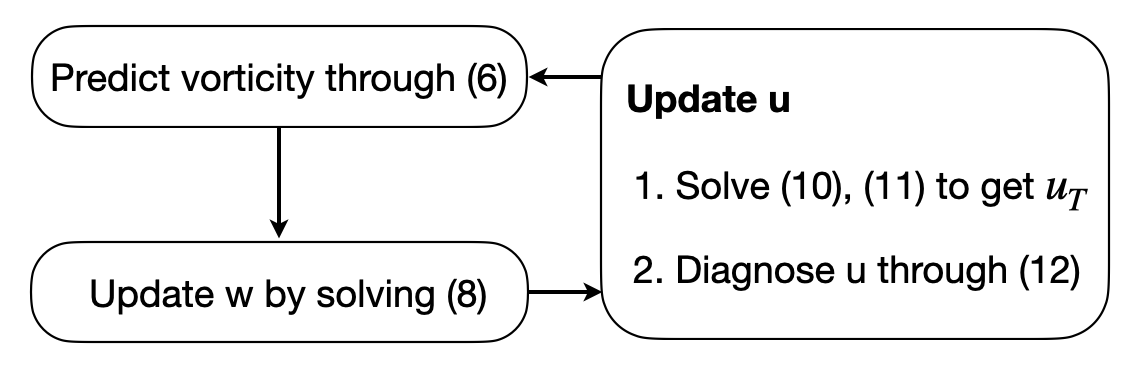
\includegraphics[width=1\textwidth] {flowchart.png}
\caption{Flowchart}
\end{figure}

Discretization 

\rule{16.5cm}{1pt}

\begin{equation*}
(6): \frac{\partial \zeta}{\partial t} = -(\frac{\partial (u\zeta)}{\partial x} + \frac{\partial (w\zeta)}{\partial z}) + \frac{\partial B}{\partial x}
\end{equation*}
\quad $u\_zeta^{n}_{i,k} = \frac{u_{i,k-1} + u_{i,k}}{2}$, $w\_zeta^{n}_{i,k} = \frac{w_{i-1,k} + w_{i,k}}{2}$, $\theta^{'} \_zeta^{n}_{i,k} = \frac{\theta^{'}_{i-1,k-1} + \theta^{'}_{i-1,k} + \theta^{'}_{i,k-1} + \theta^{'}_{i,k}}{4}$ \\\\

\quad [\_zeta means which variable's location is at zeta's place]

\begin{equation*}{}
\frac{\partial \zeta}{\partial t}: \frac{\zeta^{n+1}_{i,k} - \zeta^{n-1}_{i,k}}{2\Delta t}
\end{equation*}

\begin{equation*}{}
\frac{\partial (u\zeta)}{\partial x}: \frac{u\_zeta^{n}_{i+1,k}\times \zeta^{n}_{i+1,k} - u\_zeta^{n}_{i-1,k}\times \zeta^{n}_{i-1,k}}{2\Delta x}
\end{equation*}

\begin{equation*}{}
\frac{\partial (w\zeta)}{\partial z}: \frac{w\_zeta^{n}_{i,k+1}\times \zeta^{n}_{i,k+1} - w\_zeta^{n}_{i,k-1}\times \zeta^{n}_{i,k-1}}{2\Delta z}
\end{equation*}

\begin{equation*}{}
\frac{\partial B}{\partial x} = \frac{g}{\theta_0} \frac{\partial \theta^{'}}{\partial x} = \frac{g}{\theta_0} \times \frac{\theta^{'} \_zeta^{n}_{i+1,k} - \theta^{'} \_zeta^{n}_{i-1,k}}{2\Delta x}
\end{equation*}

\rule{16.5cm}{1pt}

\begin{equation*}
(8): \frac{\partial^2 w}{\partial x^{2}} + \frac{\partial}{\partial z}(\frac{1}{\rho_{0}}\frac{\partial (\rho_{0}w)}{\partial z}) = \frac{\partial^2 w}{\partial x^{2}} + \frac{\partial^2 w}{\partial z^{2}} + \frac{\partial}{\partial z}(\frac{w}{\rho_{0}})\frac{\partial \rho_{0}}{\partial z} + \frac{w}{\rho_{0}}\frac{\partial^2 \rho_{0}}{\partial z^{2}} = \frac{\partial \zeta}{\partial x}
\end{equation*}

\quad $\rho_{0}\_zeta^{n}_{k}$ = $\rho_{0}\_w^{n}_{k}$ = the average density at zeta and w's height ,\\

\quad $\zeta\_w^{n}_{i,k} = \frac{\zeta^{n}_{i,k+1} + \zeta^{n}_{i,k}}{2}$= value of zeta at w's location

\begin{equation*}
\frac{\partial^2 w}{\partial x^{2}}: \frac{w^{n}_{i+1,k} - 2w^{n}_{i,k} + w^{n}_{i-1,k}}{\Delta x^{2}}
\end{equation*}

\begin{equation*}
\frac{\partial^2 w}{\partial z^{2}}: \frac{w^{n}_{i,k+1} - 2w^{n}_{i,k} + w^{n}_{i,k-1}}{\Delta z^{2}}
\end{equation*}

\begin{equation*}
\frac{\partial}{\partial z}(\frac{w}{\rho_{0}})\frac{\partial \rho_{0}}{\partial z}: \frac{\frac{w^{n}_{i,k+1}}{\rho_{0}\_w^{n}_{i,k+1}} - \frac{w^{n}_{i,k-1}}{\rho_{0}\_w^{n}_{i,k-1}}}{2\Delta z} \times \frac{\rho_{0}\_w^{n}_{i,k+1} - \rho_{0}\_w^{n}_{i,k-1}}{2\Delta z} = \frac{(\rho_{0}\_w^{n}_{i,k+1} - \rho_{0}\_w^{n}_{i,k-1})(w^{n}_{i,k-1} - w^{n}_{i,k+1} + 1) }{4\Delta z^2 \rho_0\_w_{i,k+1}\rho_0\_w_{i,k-1}}
\end{equation*}\\
\newpage

\begin{equation*}
\frac{w}{\rho_{0}}\frac{\partial^2 \rho_{0}}{\partial z^{2}}: \frac{w^{n}_{i,k}}{\rho_{0}\_w^{n}_{i,k}}\frac{\rho_{0}\_w^{n}_{i,k+1} - 2\rho_{0}\_w^{n}_{i,k} + \rho_{0}\_w^{n}_{i,k-1}}{\Delta z^2}
\end{equation*}

\begin{equation*}
\frac{\partial \zeta}{\partial x}: \frac{\zeta^{n}_{i+1,k} - \zeta^{n}_{i-1,k}}{2\Delta x}
\end{equation*}

\quad $\because \Delta x = \Delta z$ \\
\begin{eqnarray*}
\Rightarrow w^{n}_{i,k}(4 - \overbrace{\frac{\rho_{0}\_w^{n}_{i,k+1} - 2\rho_{0}\_w^{n}_{i,k} + \rho_{0}\_w^{n}_{i,k-1}}{\rho^{n}_{0i,k}}}^{P}) -w^{n}_{i+1,k} - w^{n}_{i-1,k} - w^{n}_{i,k+1}(1 + \overbrace{\frac{\rho_0\_w_{i,k+1} - \rho_0\_w_{i,k-1}}{4\rho_0\_w_{i,k+1}}}^{Q}) \\ - w^{n}_{i,k-1}(1 - \underbrace{\frac{\rho_0\_w_{i,k+1} - \rho_0\_w_{i,k-1}}{4\rho_0\_w_{i,k-1}}}_{O}) = -\frac{\Delta x}{2}(\underbrace{\zeta^{n}_{i+1,k} - \zeta^{n}_{i-1,k}}_{R}) \quad (13)
\end{eqnarray*}

\begin{equation*}
A\vec{w} = \vec{b}
\end{equation*}

\begin{equation*}
1 \leq i \leq m-2, 2 \leq k \leq n-2, \vec{w} = 
\begin{bmatrix} 
	w_{12} , w_{22} , \ldots , w_{(m-2)2} , w_{13} , w_{23} , \ldots , w_{(m-2)3} , \ldots , w_{(m-2)(n-2)}
\end{bmatrix}^T
\end{equation*}

\begin{equation*}
A: (m-2)(n-3) \times (m-2)(n-3), D: (m-2) \times (m-2), E: (m-2) \times (m-2)
\end{equation*}
\begin{equation*}
F: (m-2) \times (m-2), w: (m-2)(n-3) \times 1, b: (m-2)(n-3) \times 1
\end{equation*}

\begin{equation*}
A =
\begin{bmatrix}
        ~D & E & ~0 & ~0 & ~0 & \ldots & ~0 \\
        F & ~D & E & ~0 & ~0 & \ldots & ~0 \\
        ~0 & F & ~D & E & ~0 & \ldots & ~0 \\
        \vdots & \ddots & \ddots & \ddots & \ddots & \ddots & \vdots \\
        ~0 & \ldots & ~0 & F & ~D & E & ~0 \\
        ~0 & \ldots & \ldots & ~0 & F & ~D & E \\
        ~0 & \ldots & \ldots & \ldots & ~0 & F & ~D
\end{bmatrix}, 
D = 
\begin{bmatrix}
	4-P & -1 & ~0 & ~0 & ~0 & \ldots & ~0 \\
        -1 & 4-P & -1 & ~0 & ~0 & \ldots & ~0 \\
        ~0 & -1 & 4-P & -1 & ~0 & \ldots & ~0 \\
        \vdots & \ddots & \ddots & \ddots & \ddots & \ddots & \vdots \\
        ~0 & \ldots & ~0 & -1 & 4-P & -1 & ~0 \\
        ~0 & \ldots & \ldots & ~0 & -1 & 4-P & -1 \\
        ~0 & \ldots & \ldots & \ldots & ~0 & -1 & 4-P

\end{bmatrix}
\end{equation*}


\begin{equation*}
E = 
\begin{bmatrix}
	~-1-Q & 0 & ~0 & ~0 & ~0 & \ldots & ~0 \\
        0 & ~-1-Q & 0 & ~0 & ~0 & \ldots & ~0 \\
        ~0 & 0 & ~-1-Q & 0 & ~0 & \ldots & ~0 \\
        \vdots & \ddots & \ddots & \ddots & \ddots & \ddots & \vdots \\
        ~0 & \ldots & ~0 & 0 & ~-1-Q & 0 & ~0 \\
        ~0 & \ldots & \ldots & ~0 & 0 & ~-1-Q & 0 \\
        ~0 & \ldots & \ldots & \ldots & ~0 & 0 & ~-1-Q

\end{bmatrix}
\end{equation*}

\begin{equation*}
F = 
\begin{bmatrix}
	~-1+O & 0 & ~0 & ~0 & ~0 & \ldots & ~0 \\
        0 & ~-1+O & 0 & ~0 & ~0 & \ldots & ~0 \\
        ~0 & 0 & ~-1+O & 0 & ~0 & \ldots & ~0 \\
        \vdots & \ddots & \ddots & \ddots & \ddots & \ddots & \vdots \\
        ~0 & \ldots & ~0 & 0 & ~-1+O & 0 & ~0 \\
        ~0 & \ldots & \ldots & ~0 & 0 & ~-1+O & 0 \\
        ~0 & \ldots & \ldots & \ldots & ~0 & 0 & ~-1+O

\end{bmatrix}
\end{equation*}

\newpage

\quad
$
\vec{b} =
\left[\begin{array}{l}
        -\frac{\Delta x}{2}R_{12}       \\
        -\frac{\Delta x}{2}R_{22}       \\
        -\frac{\Delta x}{2}R_{32}       \\
	~~~~~~\vdots                    \\
	-\frac{\Delta x}{2}R_{(m-2)2}   \\
        -\frac{\Delta x}{2}R_{13}       \\
        -\frac{\Delta x}{2}R_{23}       \\
        -\frac{\Delta x}{2}R_{33}       \\
        ~~~~~~\vdots                    \\
        -\frac{\Delta x}{2}R_{(m-2)3}   \\
        ~~~~~~\vdots                    \\
        -\frac{\Delta x}{2}R_{(m-2)(n-2)}
\end{array}\right]
+
\left[\begin{array}{l}
        w_{02} ~~~~~~~~~~~~~~+ w_{11}(1-O_{12})     \\
        ~~~~~~~~~~~~~~~~~~~~~~ w_{21}(1-O_{22})    \\
        ~~~~~~~~~~~~~~~~~~~~~~ w_{31}(1-O_{32})    \\
	~~~~~~~~~~~~~~~~~~~~~~~~\vdots~~~~~~~~~  \\
	w_{(m-1)2} ~~~~~~~~+ w_{(m-2)1}(1-O_{12}) \\
        w_{03} 						  \\
        			0				  \\
       				0				  \\
        ~~~~~~~~~~~~~~~~~~~~~~~~\vdots~~~~~~~~~  \\
        w_{(m-1)3}						  \\
        ~~~~~~~~~~~~~~~~~~~~~~~~\vdots~~~~~~~~~  \\
        w_{(m-1)(n-2)} + w_{(m-2)(n-1)}(1+Q_{(m-2)(n-2)})
\end{array}\right], 
$\\

$
\begin{cases}
i = 1:\qquad w_{0k} = w_{(m-2)_k}\\
i = m-2: w_{(m-1)k} = w_{1k}\\
k = 2:\qquad w_{i1}(1-O_{i2}) = 0\\
k = n-2: w_{i(n-1)}(1+Q_{i(n-2)}) = 0
\end{cases}
$\\

\begin{equation*}
A^{'}\vec{w} = \vec{c}
\end{equation*}

\begin{equation*}
A' =
\begin{bmatrix}
        ~D' & E & ~0 & ~0 & ~0 & \ldots & ~0 \\
        F & ~D' & E & ~0 & ~0 & \ldots & ~0 \\
        ~0 & F & ~D' & E & ~0 & \ldots & ~0 \\
        \vdots & \ddots & \ddots & \ddots & \ddots & \ddots & \vdots \\
        ~0 & \ldots & ~0 & F & ~D' & E & ~0 \\
        ~0 & \ldots & \ldots & ~0 & F & ~D' & E \\
        ~0 & \ldots & \ldots & \ldots & ~0 & F & ~D'
\end{bmatrix}, 
D' = 
\begin{bmatrix}
	4-P & -1 & ~0 & ~0 & ~0 & \ldots & -1 \\
        -1 & 4-P & -1 & ~0 & ~0 & \ldots & ~0 \\
        ~0 & -1 & 4-P & -1 & ~0 & \ldots & ~0 \\
        \vdots & \ddots & \ddots & \ddots & \ddots & \ddots & \vdots \\
        ~0 & \ldots & ~0 & -1 & 4-P & -1 & ~0 \\
        ~0 & \ldots & \ldots & ~0 & -1 & 4-P & -1 \\
        -1 & \ldots & \ldots & \ldots & ~0 & -1 & 4-P

\end{bmatrix}
\end{equation*}


\begin{equation*}
\vec{c} =
\begin{bmatrix}
        -\frac{\Delta x}{2}R_{11} \\
        -\frac{\Delta x}{2}R_{21} \\
        -\frac{\Delta x}{2}R_{31} \\
		~~~~~~\vdots \\
		-\frac{\Delta x}{2}R_{(m-2)1}  \\
        -\frac{\Delta x}{2}R_{12} \\
        -\frac{\Delta x}{2}R_{22} \\
        -\frac{\Delta x}{2}R_{32} \\
        ~~~~~~\vdots \\
        -\frac{\Delta x}{2}R_{(m-2)2} \\
        ~~~~~~\vdots \\
        -\frac{\Delta x}{2}R_{(m-2)(n-2)}  
\end{bmatrix}
\end{equation*}

\newpage
\begin{equation*}
(10): \frac{\partial^2 \chi}{\partial x^2} = -\frac{1}{\rho_{0}}\frac{\partial (\rho_{0}w)}{\partial z}
\end{equation*}

\begin{equation*}
w\_zeta^{n}_{i,k} = \frac{w^{n}_{i-1,k} + w^{n}_{i,k}}{2}, \quad w\_u^{n}_{i,k} = \frac{w\_zeta^{n}_{i,k+1} + w\_zeta^{n}_{i,k}}{2}
\end{equation*}

\begin{equation*}
\frac{\partial^2 \chi}{\partial x^{2}}: \frac{\chi^{n}_{i+1,k} - 2\chi^{n}_{i,k} + \chi^{n}_{i-1,k}}{\Delta x^{2}}
\end{equation*}

\begin{equation*}
-\frac{1}{\rho_{0}}\frac{\partial (\rho_{0}w)}{\partial z}: -\frac{1}{\rho^{n}_{0i,k}}\frac{\rho^{n}_{0i,k+1}w\_u^{n}_{i,k+1} - \rho^{n}_{0i,k-1}w\_u^{n}_{i,k-1}}{2\Delta z}
\end{equation*}

\begin{equation*}
\Rightarrow 2\chi^{n}_{i,k} - \chi^{n}_{i+1,k} - \chi^{n}_{i-1,k} = \frac{\Delta x}{2}\underbrace{\frac{\rho^{n}_{0i,k+1}w\_u^{n}_{i,k+1} - \rho^{n}_{0i,k-1}w\_u^{n}_{i,k-1}}{\rho^{n}_{0i,k}}}_{S}\qquad \qquad \qquad \qquad \qquad \qquad(14)
\end{equation*}
\begin{equation*}
G\vec{\chi} = \vec{h}
\end{equation*}
\begin{equation*}
1 \leq i \leq m-2, k = nz-2, \vec{\chi} = 
\begin{bmatrix} 
	\chi_{1} , \chi_{2} , \ldots , \chi_{m-2}
\end{bmatrix}^T
\end{equation*}
\begin{equation*}
G: (m-2) \times (m-2), \chi: (m-2) \times 1, h: (m-2) \times 1
\end{equation*}

\begin{equation*}
G = 
\begin{bmatrix}
	~2 & -1 & ~0 & ~0 & ~0 & \ldots & ~0 \\
        -1 & ~2 & -1 & ~0 & ~0 & \ldots & ~0 \\
        ~0 & -1 & ~2 & -1 & ~0 & \ldots & ~0 \\
        \vdots & \ddots & \ddots & \ddots & \ddots & \ddots & \vdots \\
        ~0 & \ldots & ~0 & -1 & ~2 & -1 & ~0 \\
        ~0 & \ldots & \ldots & ~0 & -1 & ~2 & -1 \\
        ~0 & \ldots & \ldots & \ldots & ~0 & -1 & ~2

\end{bmatrix}, 
\vec{h} =
\begin{bmatrix}
        \frac{\Delta x}{2}S_{1} \\
        \frac{\Delta x}{2}S_{2} \\
        \frac{\Delta x}{2}S_{3} \\
        ~~~~~~~~~\vdots ~~~ \\
        \frac{\Delta x}{2}S_{(m-2)} \\
\end{bmatrix}
+
\begin{bmatrix}
        \chi_{0}  \\
        0    	\\
        0   	\\
		\vdots  \\
	\chi_{(m-1)}  \\
        
\end{bmatrix}
if
\begin{cases}
i = 1:\qquad w_{0} = w_{(m-2)}\\
i = m-2: w_{(m-1)} = w_{1}\\

\end{cases}
\end{equation*}

\begin{equation*}
G'\vec{\chi} = \vec{h'}
\end{equation*}
\begin{equation*}
G' = 
\begin{bmatrix}
        ~2 & -1 & ~0 & ~0 & ~0 & \ldots & -1 \\
        -1 & ~2 & -1 & ~0 & ~0 & \ldots & ~0 \\
        ~0 & -1 & ~2 & -1 & ~0 & \ldots & ~0 \\
        \vdots & \ddots & \ddots & \ddots & \ddots & \ddots & \vdots \\
        ~0 & \ldots & ~0 & -1 & ~2 & -1 & ~0 \\
        ~0 & \ldots & \ldots & ~0 & -1 & ~2 & -1 \\
        -1 & \ldots & \ldots & \ldots & ~0 & -1 & ~2

\end{bmatrix}
, \quad
h' = 
\begin{bmatrix}
        \frac{\Delta x}{2}S_{1} \\
        \frac{\Delta x}{2}S_{2} \\
        \frac{\Delta x}{2}S_{3} \\
        ~~~~~~~~~\vdots ~~~ \\
        \frac{\Delta x}{2}S_{(m-2)} \\

\end{bmatrix}
\end{equation*}

\newpage

\begin{equation*}
u_{\chi} = \frac{\partial \chi}{\partial x} = \frac{\chi^{n}_{i+1,k} - \chi^{n}_{i-1,k}}{2\Delta x}
\end{equation*}

\begin{equation*}
u = \int_{z_{T}}^{z}(\frac{\partial w}{\partial x} - \zeta)dz + u_{T}
\end{equation*}

\begin{equation*}
u^{n}_{i,k} = (\frac{w^{n}_{i+1,k} - w^{n}_{i-1,k}}{2\Delta x}-\zeta_{i,k})\times z - (\frac{w^{n}_{i+1,nz-1} - w^{n}_{i-1,nz-1}}{2\Delta x}-\zeta_{i,nz-1})\times z + u_{\chi}
\end{equation*}

\begin{equation*}
\frac{\partial \theta}{\partial t} = -(u\frac{\partial \theta}{\partial x} + \frac{1}{\rho_{0}}\frac{\partial\rho_{0} w \theta}{\partial z}) 
\end{equation*}

\begin{equation*}
\frac{\partial \theta}{\partial t}: \frac{\theta^{n+1}_{i,k} - \theta^{n-1}_{i,k}}{2\Delta t}
\end{equation*}

\begin{equation*}
u \frac{\partial\theta}{\partial x}: u\_th^{n}_{i,k}\frac{\theta^{n}_{i+1,k} - \theta^{n}_{i-1,k}}{2\Delta x}
\end{equation*}

\begin{equation*}
\frac{1}{\rho_{0}}\frac{\partial \rho_{0}w\theta^{'}}{\partial z}: \frac{1}{\rho_{0k}}\frac{\rho_{0k+1}w\_th^{n}_{i,k+1}\theta^{'n}_{i,k+1} - \rho_{0k-1}w\_th^{n}_{i,k-1}\theta^{'n}_{i,k-1}}{2\Delta z}
\end{equation*}


\end{CJK*}
\end{document}